\documentclass{article}
\usepackage[utf8]{inputenc}

\title{Mondes 3D - TD 1}
\author{Arnaud Gallardo}
\date{26 Janvier 2017}

\usepackage{natbib}
\usepackage{graphicx}

\usepackage{pgf,tikz}
\usepackage{mathrsfs}
\usepackage{amsmath}

\usetikzlibrary{arrows}

\begin{document}

\maketitle

\section{Rayons primaires}
\paragraph*{}
La mise en place de ces premiers rayons n'a posée aucun problème difficile à
résoudre. Les résultats sont cohérents avec ceux présentés dans l'énoncé.

\subsection*{Résultats}
\begin{figure}[htb!]
\centering
\begin{minipage}{.45\textwidth}
  \centering
  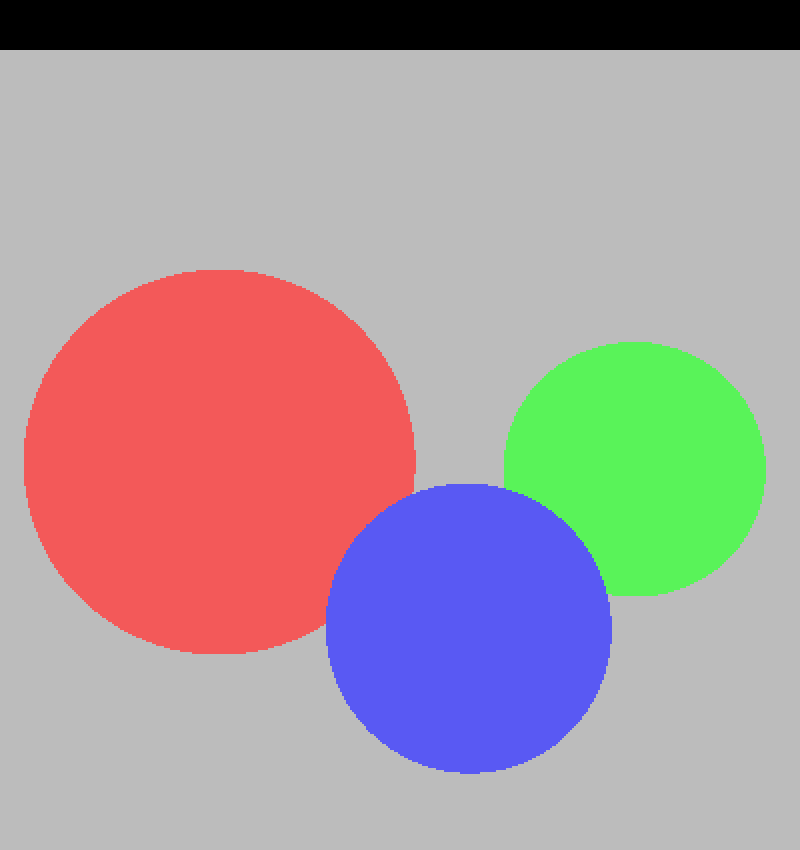
\includegraphics[width=\linewidth]{results/troisSpheres_flat.png}
  \caption{Trois sphères - Flat}
  \label{fig:tsflat}
\end{minipage}\hfill
\begin{minipage}{.45\textwidth}
  \centering
  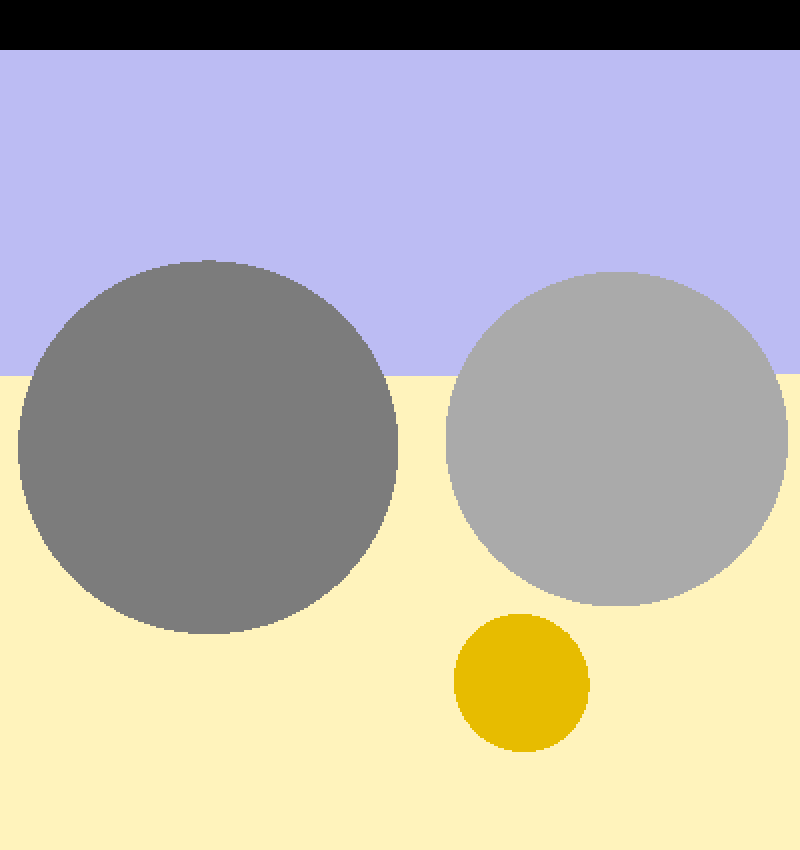
\includegraphics[width=\linewidth]{results/petanque_flat.png}
  \caption{Pétanque - Flat}
  \label{fig:pflat}
\end{minipage}
\end{figure}


\section{Éclairage local}
\paragraph*{}
De même que pour la première partie, l'implémentation de l'éclairage local n'a
pas vraiment posé de problème. Seuls l'oubli de certaines normalisations de vecteurs
et quelques erreurs lors de la transformation des fonctions mathématiques en code
ont entraînés des bugs facilement résolus.\\
Ici aussi, les résultats obtenus correspondent aux resultats attendus.

\subsection*{Résultats}
\begin{figure}[htb!]
\centering
\begin{minipage}{.45\textwidth}
  \centering
  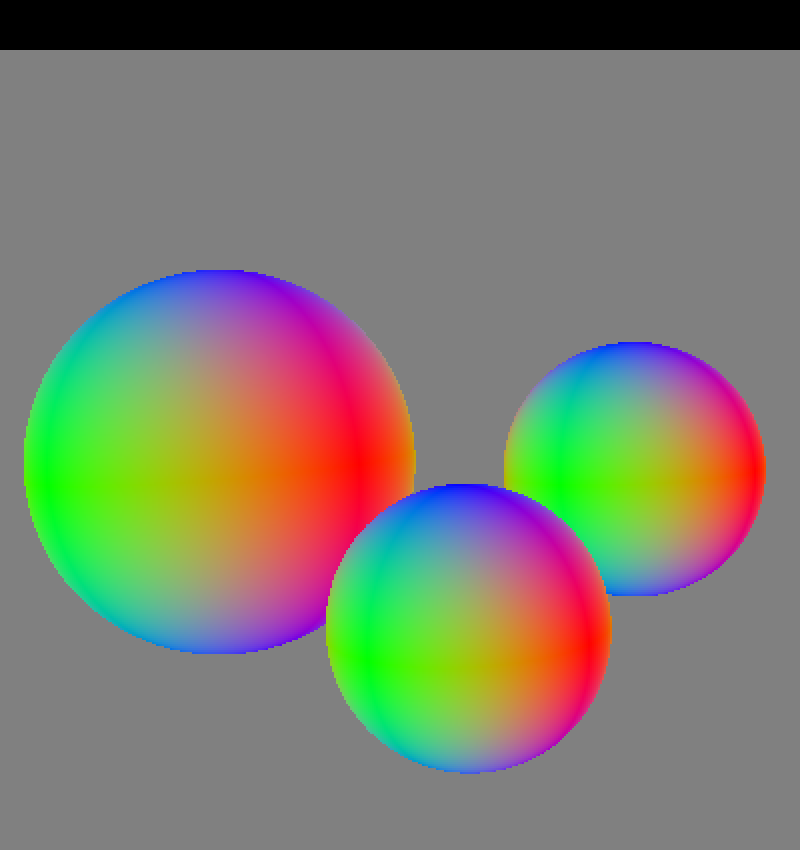
\includegraphics[width=\linewidth]{results/troisSpheres_normals.png}
  \caption{Normales sur trois sphères}
  \label{fig:tsnormal}
\end{minipage}\hfill
\begin{minipage}{.45\textwidth}
  \centering
  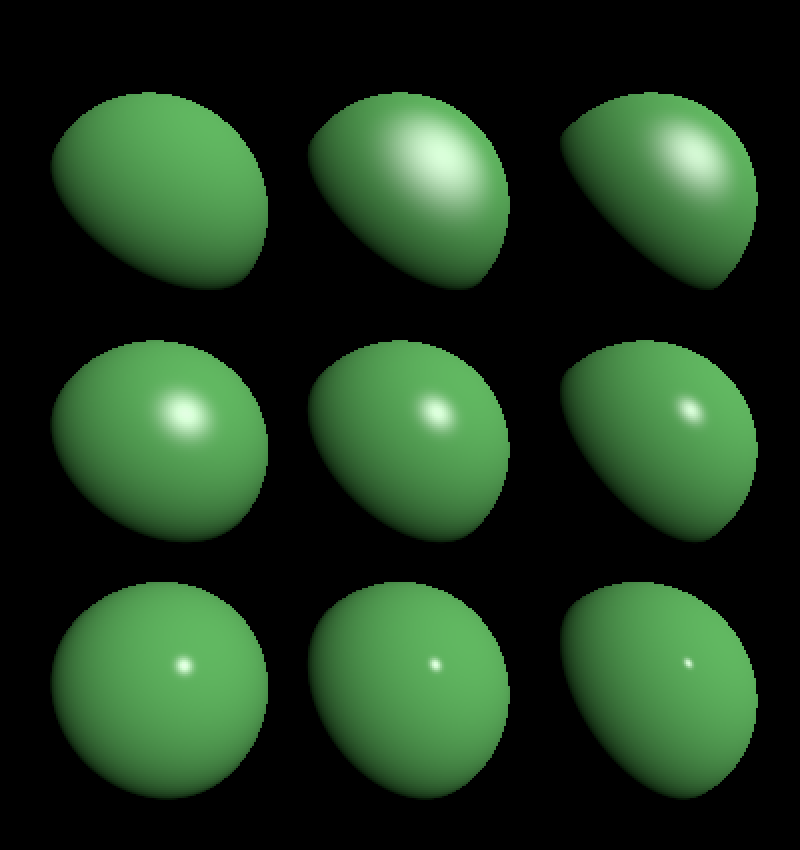
\includegraphics[width=\linewidth]{results/phong_direct.png}
  \caption{BRDF de Phong}
  \label{fig:phdirect}
\end{minipage}
\end{figure}



\section{Rayons secondaires}
\paragraph*{}
Lors de l'implémentation des ombres portées et des rebonds multiples, je me suis
heurté à un plusieurs problèmes :\\

\subsubsection*{Vérifier si l'objet détecté comme bloquant la lumière est bien entre la
source et l'objet recevant la lumière}
L'énoncé conseille de \textit{"comparer le temps d'intersection avec la distance
à la lampe"} or la distance a la lampe n'est pas immédiatement disponible, il
faudrait modifier la classe \textit{pointLight} afin d'accèder à la position
 de la lampe. \\
 J'utilise donc une méthode différente afin de savoir si l'objet bloquant est
 bien entre l'objet et la lumière.\\
 On appelle \textit{pointObjet} le point sur l'objet dont on veut
 déterminer la couleur et \textit{pointHit} le point d'impact renvoyé par notre rayon.
 On calcule \textit{directionObjet} et \textit{directionHit} à l'aide de la
 fonction \textbf{pointLight.direction(point[...])}.\\

\definecolor{ffvvqq}{rgb}{1.,0.3333333333333333,0.}
\definecolor{qqqqff}{rgb}{0.,0.,1.}
\begin{tikzpicture}[line cap=round,line join=round,>=triangle 45,x=0.5cm,y=0.5cm]
\clip(-6.407328215765398,0.6138053348705027) rectangle (15.730080498252612,11.300830231292991);
\draw(-4.78,4.48) circle (0.7144928271158502cm);
\draw(0.44,5.34) circle (0.3551056180912941cm);
\draw [line width=1.2pt,dash pattern=on 3pt off 3pt,domain=-3.5797711299683272:15.730080498252612] plot(\x,{(--52.1373011724171--1.0725596155870853*\x)/9.189893358955564});
\draw [-latex,line width=1.2pt,color=ffvvqq] (-3.5797711299683272,5.25553250063585) -- (-1.8612804147486215,5.45609889122512);
\draw [-latex,line width=1.2pt, color=ffvvqq] (-0.19892860475988794,5.650113266435961) -- (1.4578443737520828,5.8434765318775765);
\begin{scriptsize}
\draw[color=black] (-4.9024206283099865,4.594176852415613) node {$objet$};
\draw [color=qqqqff] (-3.5797711299683272,5.25553250063585)-- ++(-2.5pt,-2.5pt) -- ++(5.0pt,5.0pt) ++(-5.0pt,0) -- ++(5.0pt,-5.0pt);
\draw[color=qqqqff] (-3.1576002370573355,5.880981890964443) node {$pointObjet$};
\draw [color=qqqqff] (5.610122228987237,6.328092116222935)-- ++(-2.5pt,-2.5pt) -- ++(5.0pt,5.0pt) ++(-5.0pt,0) -- ++(5.0pt,-5.0pt);
\draw[color=qqqqff] (5.653742738768553,6.862443361044059) node {$pointLight$};
\draw[color=black] (0.2011790161040179,4.310643538837057) node {$objetBloquant$};
\draw [color=qqqqff] (-0.19892860475988794,5.650113266435961)-- ++(-1.5pt,-1.5pt) -- ++(3.0pt,3.0pt) ++(-3.0pt,0) -- ++(3.0pt,-3.0pt);
\draw[color=qqqqff] (0.26660978077599246,5.4229665382606225) node {$pointHit$};
\draw[color=ffvvqq] (-2.3288105512123263,4.877710165994169) node {$directionObjet$};
\draw[color=ffvvqq] (0.8554866628237621,6.491669027902871) node {$directionHit$};
\end{scriptsize}
\end{tikzpicture}

Dans ce premier cas, \textit{directionObjet} et \textit{directionHit} sont
identiques (et par définition normalisés), on a donc :\\

$$<directionObjet \cdot directionHit>$$
$$= <directionObjet \cdot directionObjet>$$
$$= <directionHit \cdot directionHit>$$
$$= ||directionObjet||^2$$
$$= 1^2 = 1$$

\begin{tikzpicture}[line cap=round,line join=round,>=triangle 45,x=0.5cm,y=0.5cm]
\clip(-6.407328215765398,0.6138053348705027) rectangle (15.730080498252612,11.300830231292991);
\draw(-4.78,4.48) circle (0.7144928271158502cm);
\draw(8.727896858450093,6.081548666282377) circle (0.3551056180912955cm);
\draw [line width=1.2pt,dash pattern=on 3pt off 3pt,domain=-3.5797711299683272:15.730080498252612] plot(\x,{(--52.1373011724171--1.0725596155870853*\x)/9.189893358955564});
\draw [-latex,line width=1.2pt,color=ffvvqq] (-3.5797711299683272,5.25553250063585) -- (-1.8612804147486215,5.45609889122512);
\draw [-latex,color=ffvvqq] (8.290249523089116,6.640891861334784) -- (6.589866492188188,6.442438832693636);
\begin{scriptsize}
\draw[color=black] (-4.9024206283099865,4.594176852415613) node {$objet$};
\draw [color=qqqqff] (-3.5797711299683272,5.25553250063585)-- ++(-2.5pt,-2.5pt) -- ++(5.0pt,5.0pt) ++(-5.0pt,0) -- ++(5.0pt,-5.0pt);
\draw[color=qqqqff] (-3.1576002370573355,5.880981890964443) node {$pointObjet$};
\draw [color=qqqqff] (5.610122228987237,6.328092116222935)-- ++(-2.5pt,-2.5pt) -- ++(5.0pt,5.0pt) ++(-5.0pt,0) -- ++(5.0pt,-5.0pt);
\draw[color=qqqqff] (4.846763307814202,5.880981890964443) node {$pointLight$};
\draw[color=black] (8.48907587455411,5.052192205119434) node {$objetBloquant$};
\draw [color=qqqqff] (8.290249523089116,6.640891861334784)-- ++(-1.5pt,-1.5pt) -- ++(3.0pt,3.0pt) ++(-3.0pt,0) -- ++(3.0pt,-3.0pt);
\draw[color=qqqqff] (8.75079893324201,6.404428008340238) node {$pointHit$};
\draw[color=ffvvqq] (-2.3288105512123263,4.877710165994169) node {$directionObjet$};
\draw[color=ffvvqq] (6.918737522426725,7.102356164841299) node {$directionHit$};
\end{scriptsize}
\end{tikzpicture}

Dans le deuxième cas, \textit{directionObjet} et \textit{directionHit} sont
opposé (et par définition normalisés), on a donc :\\

$$<directionObjet \cdot directionHit>$$
$$= -||directionObjet||\cdot||directionHit||$$
$$= -1*1 = -1$$

On peut donc utiliser le produit scalaire de \textit{directionObjet} et
\textit{directionHit} afin de vérifier que l'objet bloquant est réellement bloquant
(si le produit scalaire retourne 1 alors l'objet bloque bien la lumière).

De plus, il n'est plus nécessaire de séparer le cas de \textbf{directionLight}
qui renvoi toujours la même direction et donc se retrouve toujours dans le premier cas.

Avant de comparer le résultat de ce produit scalaire à \textit{-1}, j'utilise la
fonction \textbf{round} pour éviter les problèmes d'égalités de \textit{floats}.\\

\subsubsection*{Accèder à la valeur de \textit{maxRecursion}}
Je n'ai pas réussi à acceder à la valeur de \textit{maxRecursion} lors de
l'instanciation du premier rayon. J'ai donc décidé de changer la valeur par
défaut de \textit{recursionLevel} dans la classe \textbf{Ray} en $-1$, afin de
pouvoir reconnaitre facilement la première utilisation du rayon dans l'integrator
et fixer le bon niveau de recursion.

\subsubsection*{Problèmes restants}
J'observe encore deux résultats différents de ceux attendus :
\begin{itemize}
\item Sur la scène \textit{petanque.scn}, le plan bleu n'apparait pas.
\item Sur la scène \textit{troisSpheres.scn}, les sphères apparaisent plus claires
que sur le TD. Si on change la couleur du fond en noir (donc que l'on enlève
l'effet du backgroundColor sur les rayons secondaires...) alors les couleurs semblent correspondre.
\end{itemize}

\subsection*{Résultats}
\begin{figure}[htb!]
\centering
\begin{minipage}{.45\textwidth}
  \centering
  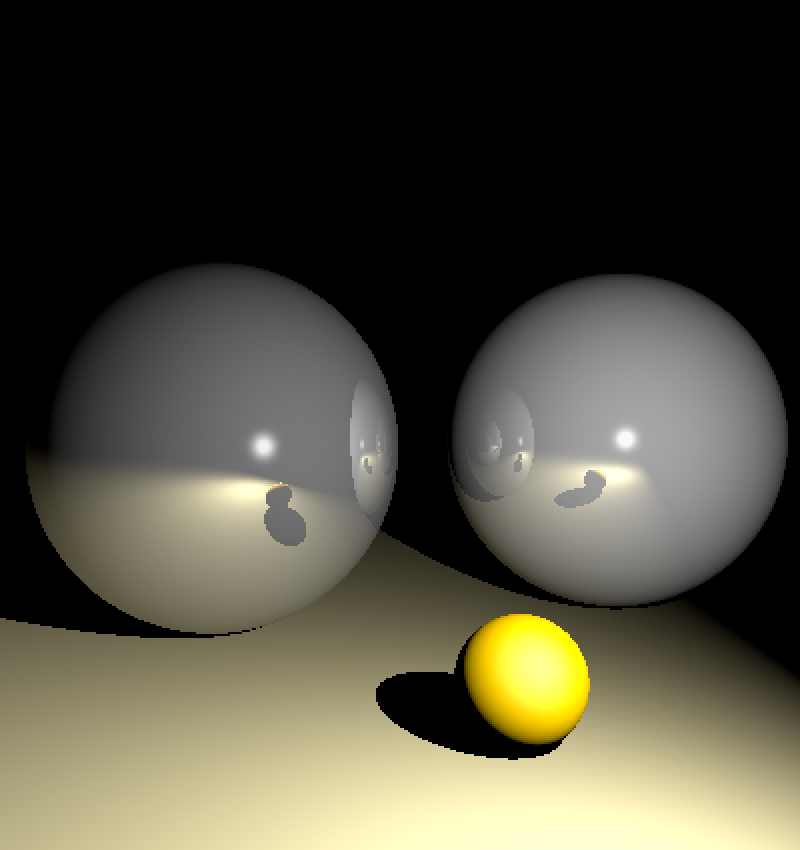
\includegraphics[width=\linewidth]{results/petanque_whitted.png}
  \caption{Pétanque - Whitted}
  \label{fig:tsnormal}
\end{minipage}\hfill
\begin{minipage}{.45\textwidth}
  \centering
  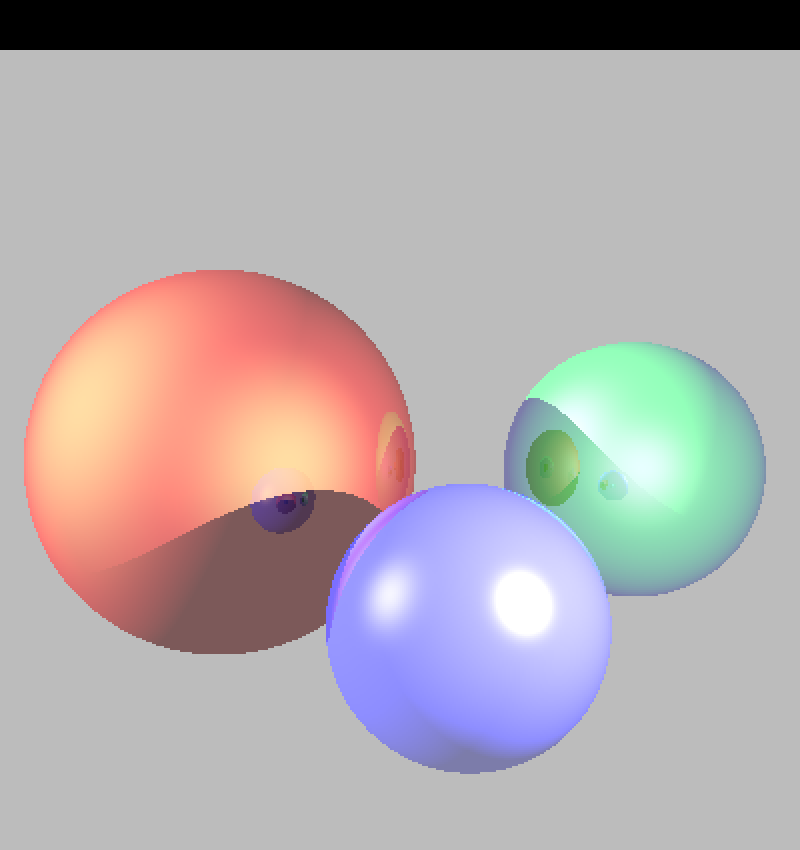
\includegraphics[width=\linewidth]{results/troisSpheres_whitted.png}
  \caption{Trois sphères, fond gris}
  \label{fig:phdirect}
\end{minipage}
\end{figure}

\begin{figure}[htb!]
\centering
\begin{minipage}{.45\textwidth}
  \centering
  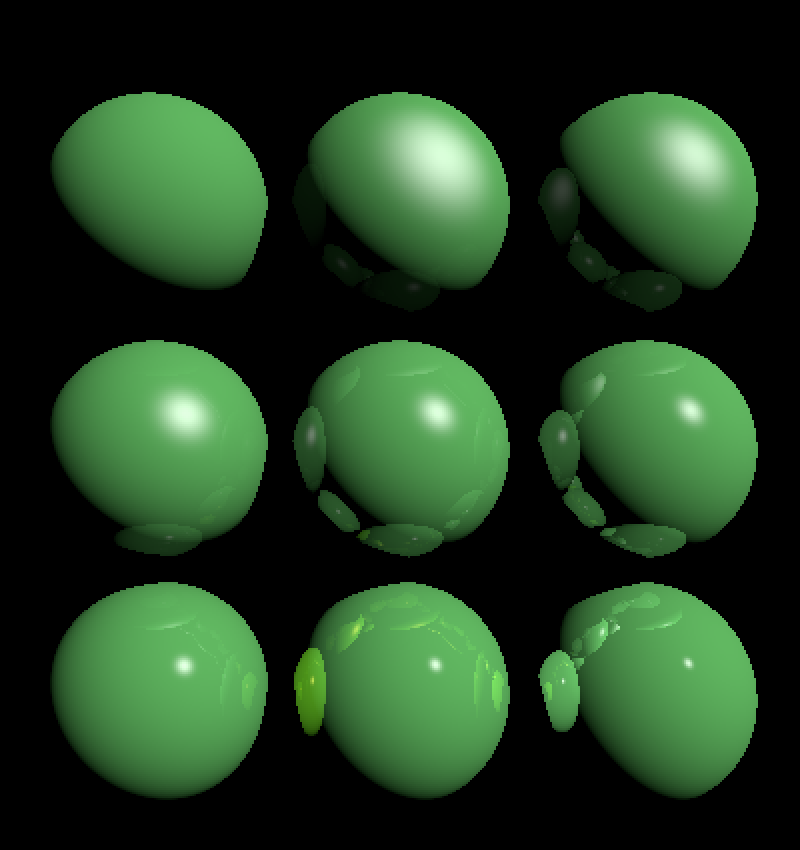
\includegraphics[width=\linewidth]{results/phong_whitted.png}
  \caption{Phong - Whitted}
  \label{fig:tsnormal}
\end{minipage}\hfill
\begin{minipage}{.45\textwidth}
  \centering
  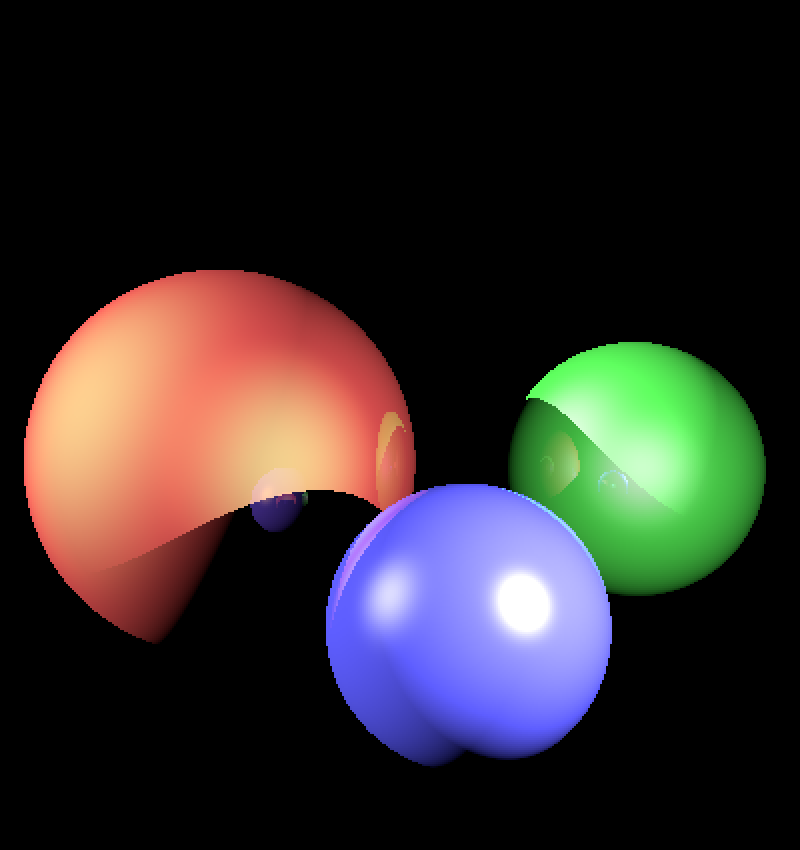
\includegraphics[width=\linewidth]{results/troisSpheres_whitted_NoBG.png}
  \caption{Trois sphères, fond noir}
  \label{fig:phdirect}
\end{minipage}
\end{figure}

\end{document}
